% ============================================================================
%  Capítulo 6 - Comparación PID ISA contra ADRC
% ============================================================================
\chapter{Comparación PID ISA contra ADRC}
\label{cap:comparacion_pid}
En este capítulo se compara un PID ISA ideal, con filtro en la acción derivativa, con el ADRC de los
capítulos anteriores, bajo un mismo grado de robustez, y se mide su desempeño con métricas clásicas,
para ver en qué casos el ADRC puede llegar a ser más beneficioso de implementar que el PID y qué
ventajas y desventajas tiene frente a un PID convencional. Para ello también se usa la perturbación
total medida en M2 en la Sección~\ref{sec:ident_perturbacion}.
%--------------------------------------------------------------------
\section{PID con misma robustez}
\label{sec:pid_robustez}

Se usa un PID ISA ideal con filtro en la acción derivativa, que actúa sobre el mismo error que el ADRC,
$e = r - y = -e_y$:
\begin{equation}
C_{PID}(s) = K_p\left(1 + \frac{1}{T_i\,s} + \frac{T_d\,s}{1 + \dfrac{T_d}{N}\,s}\right),
\label{eq:pid_isa}
\end{equation}
con $K_p$ la ganancia proporcional, $T_i$ el tiempo integral, $T_d$ el tiempo
derivativo y $N$ el que fija el filtro de la derivada.

\paragraph{Sintonía.} El PID se sintoniza en dos pasos. Primero se elige $K_p$ para que la señal de
control no salte de forma exagerada en el cambio de consigna. Ante un escalón $\Delta r$, la acción resultante es $K_p\,(1 + N)\,\Delta r$. Se busca un salto de cerca de $40~\%$ ante el
escalón de $0{,}2$~mg/L, de $40$ a $80~\%$, el mismo pico de la señal de control del ADRC. Con el valor
típico $N = 10$ queda un $K_p$ pequeño: la acción proporcional, que es la que mueve la salida al inicio
y rechaza las perturbaciones, sería tan débil que el controlador quedaría casi sin fuerza para rechazar
la perturbación y muy lento. Por eso se usa $N = 2$, que deja más acción proporcional para el mismo
salto. Luego se ajustan las acciones integral y derivativa para que el PID tenga, sin retardo, la misma
sensibilidad máxima $M_s$ que el ADRC. El retardo $\theta = 50$~s solo se usa para evaluar. Resulta
\begin{equation}
K_p = 66{,}7~\%/(\mathrm{mg/L}),
\qquad
T_i = 160{,}9~\mathrm{s},
\qquad
T_d = 40{,}2~\mathrm{s},
\qquad
N = 2 .
\label{eq:pid_ganancias}
\end{equation}
Con la misma $M_s$, el PID queda con un ancho de banda menor que el del ADRC, porque el salto inicial
limita su ganancia, y en la Figura~\ref{fig:pid_adrc_sensibilidad}(a) se ve que su pico de sensibilidad
está en una frecuencia mucho más baja. Es decir, para esta misma configuración el ADRC puede rechazar
perturbaciones de frecuencias mucho más altas que el PID. Con $\theta = 50$~s los dos quedan con casi el
mismo margen de fase; el PID pierde menos robustez al usar la planta con retardo y tiene un mayor margen
de ganancia, pero es más lento (Tabla~\ref{tab:pid_robustez} y Figura~\ref{fig:pid_adrc_escalon}).

\begin{table}[H]
\centering
\caption[Robustez del ADRC y del PID ISA]{Robustez del ADRC y del PID ISA (Tabla~\ref{tab:metricas_robustez}), sin
  retardo (diseño) y con $\theta = 50$~s (evaluación).}
\label{tab:pid_robustez}
\renewcommand{\arraystretch}{1.3}
\begin{tabular}{llccccc}
\toprule
 & $\boldsymbol{\theta}$ & $\boldsymbol{M_s}$ & $\boldsymbol{M_t}$ &
 \textbf{MF} & \textbf{MG} & $\boldsymbol{\omega_{BW}}$ \textbf{[rad/h]} \\
\midrule
ADRC & 0     & 1,202 & 1,100 & $65{,}8^{\circ}$ & $\infty$ & 56,4 \\
PID  & 0     & 1,202 & 1,418 & $50{,}0^{\circ}$ & $\infty$ & 21,2 \\
\midrule
ADRC & 50~s  & 2,318 & 1,700 & $36{,}0^{\circ}$ & 2,12     & 79,0 \\
PID  & 50~s  & 1,585 & 1,709 & $37{,}5^{\circ}$ & 7,37     & 23,8 \\
\bottomrule
\end{tabular}
\end{table}

\begin{figure}[H]
  \centering
  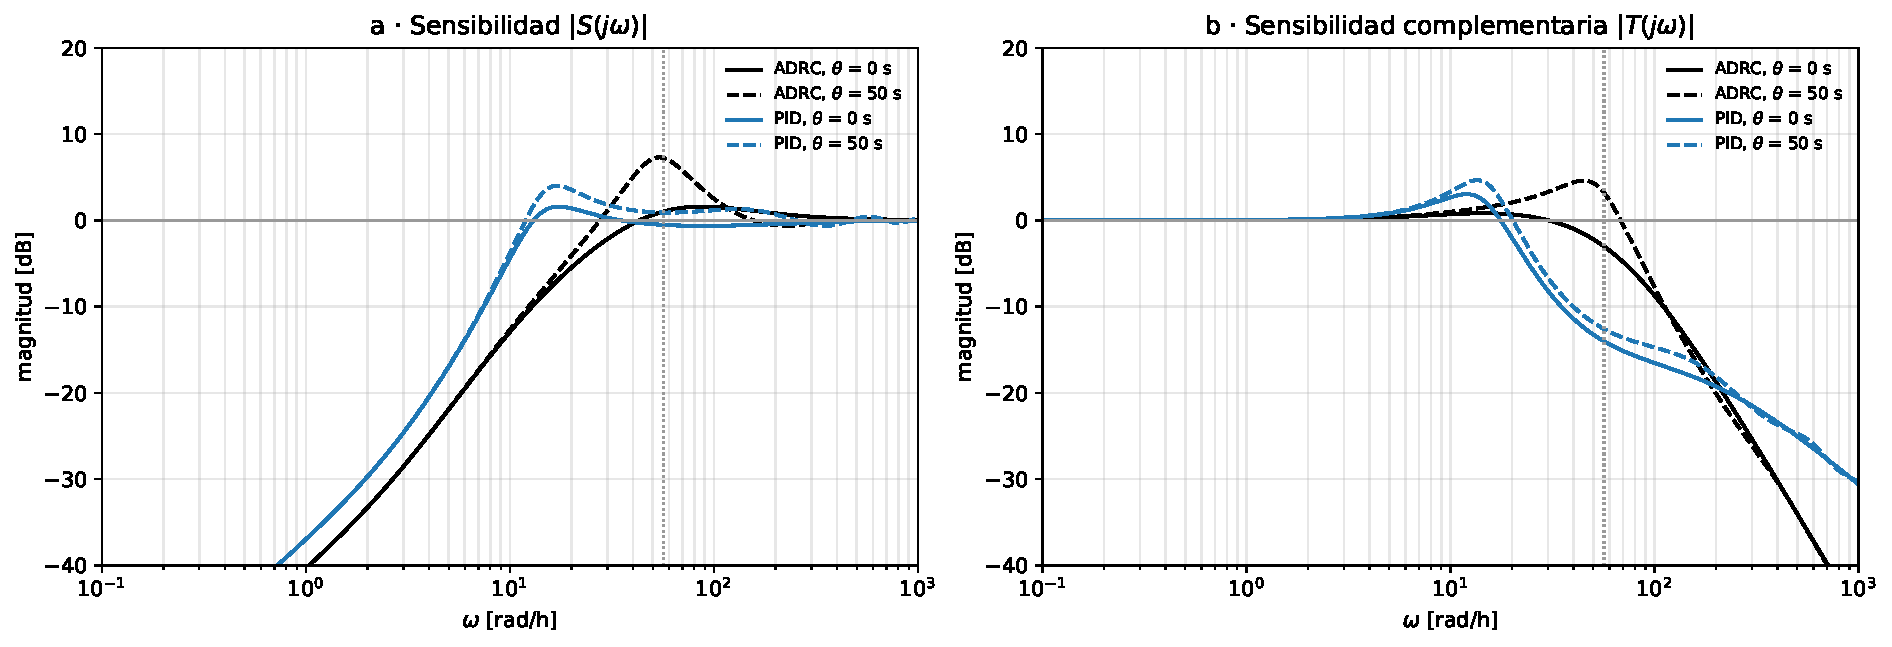
\includegraphics[width=\textwidth]{pid_adrc_sensibilidad.pdf}
  \caption[Sensibilidad del ADRC y del PID ISA]{Sensibilidad del ADRC y del PID
    ISA sin retardo (continua) y con $\theta = 50$~s (discontinua): (a)
    $|S(j\omega)|$ y (b) $|T(j\omega)|$. La vertical punteada marca
    el $\omega_{BW}$ del ADRC.}
  \label{fig:pid_adrc_sensibilidad}
\end{figure}

\paragraph{Escalón de consigna.} Se aplica el cambio de $2{,}0$ a
$2{,}2$~mg/L, sin retardo, que es el caso de diseño, y con $\theta = 50$~s
(Figura~\ref{fig:pid_adrc_escalon}), con el ruido del sensor
de la Sección~\ref{sec:ident_ruido} ($\sigma = 0{,}0011$~mg/L, blanco, a 50~ms)
sumado a la medida. El soplador se limita entre $0$ y $100~\%$: el ADRC
realimenta $b_0\,u_{\mathrm{sat}}$ al observador, y el PID usa el mismo esquema de anti-\emph{windup}
que el GPI \eqref{eq:aw_gpi} \cite[ec.~19.3]{levine2011handbook}. Con
este escalón ninguno de los dos llega al límite del soplador: el pico del ADRC es
de $80~\%$ sin retardo y de $93~\%$ con $\theta = 50$~s, y el del PID es de
$80~\%$ en los dos casos. La Tabla~\ref{tab:pid_escalon} reúne las métricas de la
Tabla~\ref{tab:metricas}: IAE, ITAE, $M_p$, $t_s$, los valores extremos de $u$, la variación total TV y
$\sigma_u$, esta última con el sistema en estacionario.

\begin{figure}[H]
  \centering
  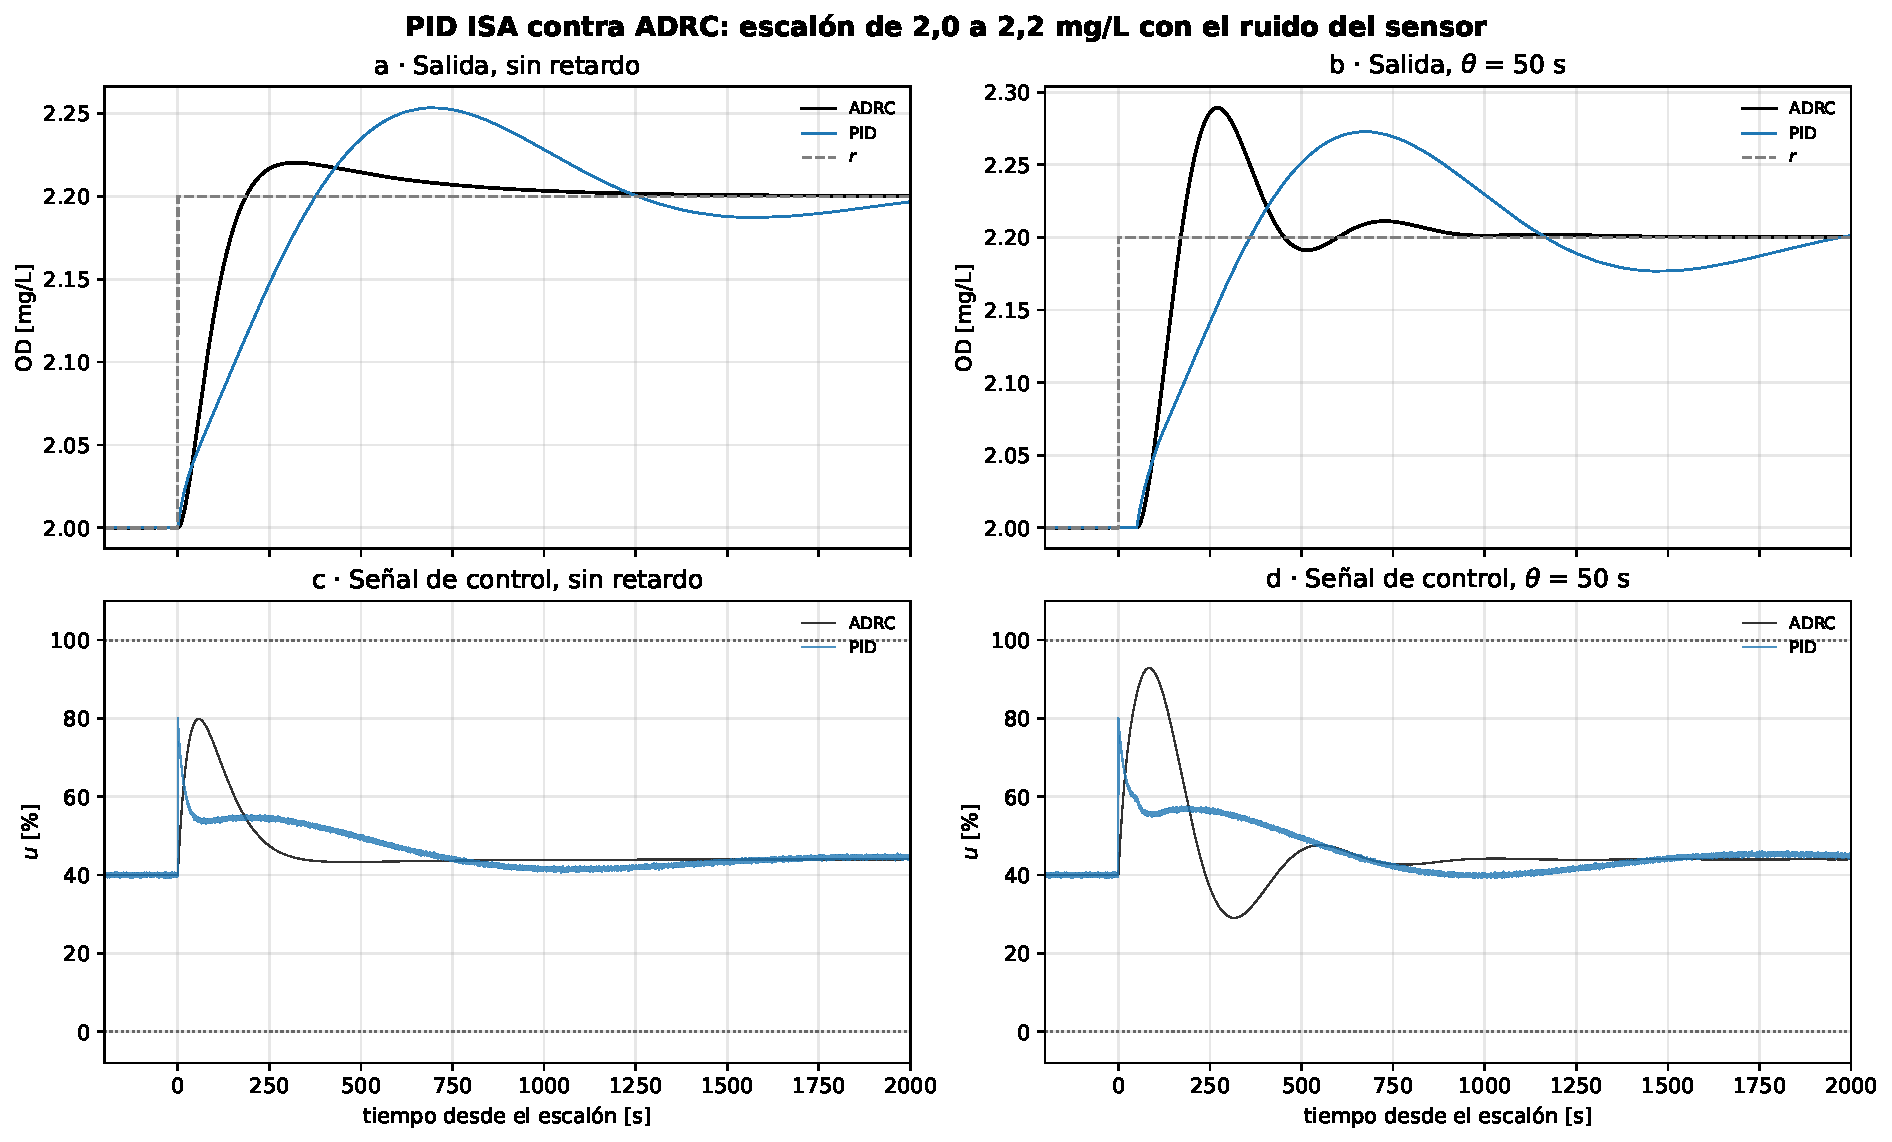
\includegraphics[width=\textwidth]{pid_adrc_escalon.pdf}
  \caption[PID ISA contra ADRC: escalón de consigna]{PID ISA contra ADRC en el escalón de $2{,}0$ a
    $2{,}2$~mg/L con el ruido del sensor y el soplador limitado entre $0$ y $100~\%$. (a) y (c) Salida y
    señal de control sin retardo; (b) y (d) con $\theta = 50$~s.}
  \label{fig:pid_adrc_escalon}
\end{figure}

\begin{table}[H]
\centering
\caption[Índices del escalón de consigna]{Índices del escalón de $2{,}0$ a
  $2{,}2$~mg/L sin retardo y con $\theta = 50$~s.}
\label{tab:pid_escalon}
\renewcommand{\arraystretch}{1.3}
\resizebox{\textwidth}{!}{%
\begin{tabular}{llccccccc|cc}
\toprule
 & & \multicolumn{7}{c|}{\textbf{Sin ruido}} & \multicolumn{2}{c}{\textbf{Con ruido}} \\
 & $\boldsymbol{\theta}$ & \textbf{IAE} & \textbf{ITAE} & $\boldsymbol{M_p}$ & $\boldsymbol{t_s}$ &
 $\boldsymbol{u_{\max}}$ & $\boldsymbol{u_{\min}}$ &
 \textbf{TV} & $\boldsymbol{\sigma_u}$ & \textbf{TV} \\
 & [s] & [mg$\cdot$s/L] & [mg$\cdot$s$^2$/L] & [\%] & [min] & [\%] & [\%] & [\%] & [\%] & [\%] \\
\midrule
ADRC & 0  & 26,9 & 6\,909  & 10,2 & 15,7   & 79,8 & 40,0 & 77  & 0,009 & 96 \\
PID  & 0  & 69,2 & 40\,127 & 26,7 & 32,9   & 80,0 & 40,0 & 84  & 0,220 & 13\,876 \\
\midrule
ADRC & 50 & 42,7 & 9\,308  & 44,6 & 14,7   & 92,8 & 29,0 & 142 & 0,010 & 158 \\
PID  & 50 & 88,4 & 56\,567 & 36,4 & 42,7   & 80,0 & 39,9 & 90  & 0,220 & 13\,873 \\
\bottomrule
\end{tabular}%
}
\end{table}

Sin retardo, con la misma sensibilidad y sin que la señal de control llegue a la saturación, el PID
es un poco más lento y tiene un sobrepico más grande, es decir, un desempeño algo peor que el del ADRC
(Figura~\ref{fig:pid_adrc_escalon}(a)). Además, en la
Figura~\ref{fig:pid_adrc_escalon}(c) ya se alcanza a ver el ruido que el PID deja pasar a la
señal de control, porque es bipropio (Sección~\ref{sec:impl_ruido}), mientras que el ADRC casi no lo deja
pasar. Cuando se introduce el retardo (Figura~\ref{fig:pid_adrc_escalon}(b) y (d)), el ADRC empieza a oscilar; el
PID, como ya era lento, no oscila tanto, pero tampoco tiene un buen desempeño y tarda mucho más en
asentarse. De hecho, con el retardo de la planta los dos tienen casi el mismo margen de fase
(Tabla~\ref{tab:pid_robustez}), pero el PID tiene un mayor margen de ganancia, pagando con un sistema
más lento. Ahora bien, el desempeño del ADRC es mejor, con un IAE y un ITAE mucho menores, tanto sin
retardo como con retardo y con la misma $M_s$; con retardo el PID queda con mejor $M_s$. El otro tema es el ruido: en la Figura~\ref{fig:pid_adrc_escalon} y en la
Tabla~\ref{tab:pid_escalon} se ve que el ruido que alcanza a pasar a la señal de control es mucho mayor
en el PID que en el ADRC.

%--------------------------------------------------------------------
\section{Perturbación de entrada}
\label{sec:pid_perturbacion_escalon}

Con el sistema en estacionario en $2{,}0$~mg/L entra una perturbación de entrada $\varepsilon = -15~\%$, una
pérdida de eficiencia del soplador, sin retardo y con $\theta = 50$~s
(Figura~\ref{fig:pid_adrc_perturbacion_escalon}). La Tabla~\ref{tab:pid_pert_escalon} reúne el IAE, la
caída máxima del OD y cuánto se pasa la salida por encima de la consigna al recuperarse, en porcentaje
de la caída (Tabla~\ref{tab:metricas}).

\begin{figure}[H]
  \centering
  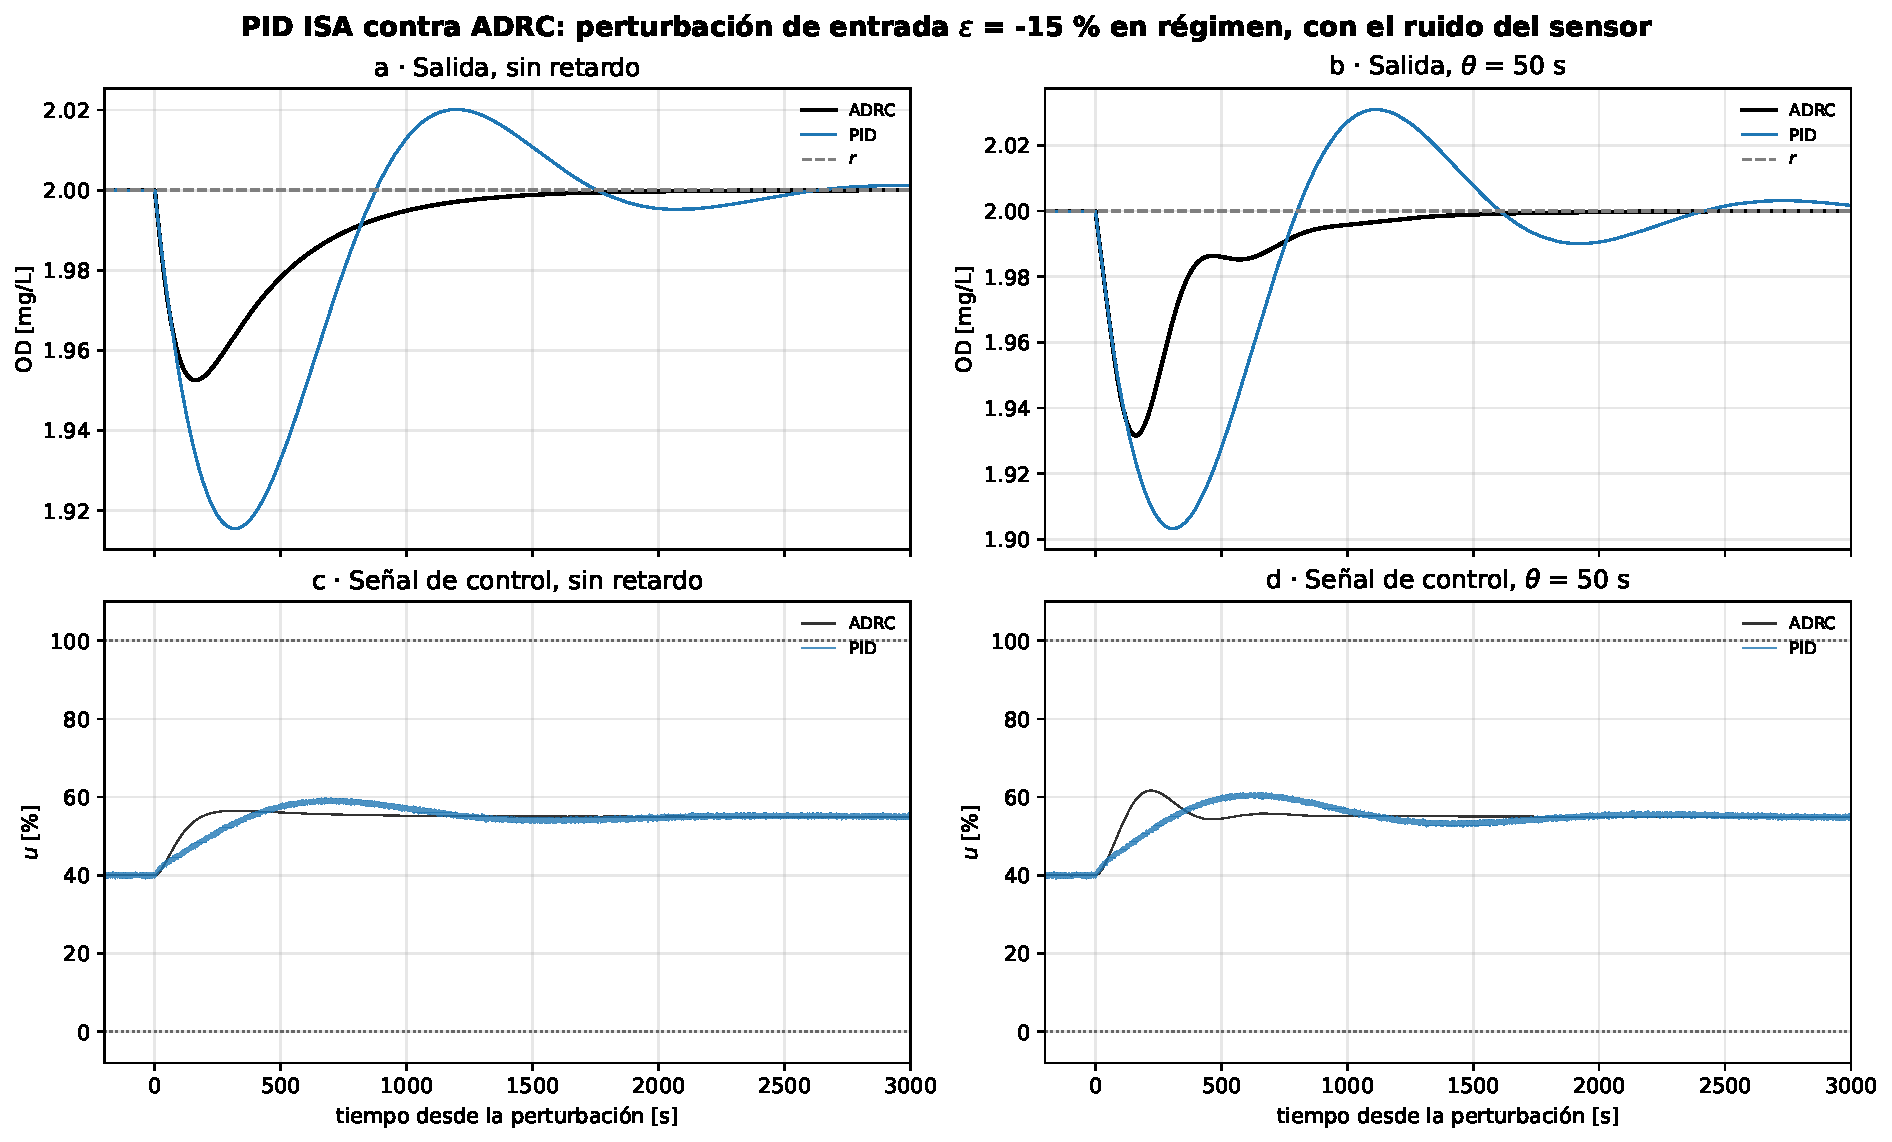
\includegraphics[width=\textwidth]{pid_adrc_perturbacion_escalon.pdf}
  \caption[PID ISA contra ADRC: perturbación de entrada]{PID ISA contra ADRC ante una perturbación de
    entrada $\varepsilon = -15~\%$ con el sistema en estacionario en $2{,}0$~mg/L, el ruido del sensor y el soplador
    limitado entre $0$ y $100~\%$. (a) y (c) Salida y señal de control sin retardo; (b) y (d) con
    $\theta = 50$~s.}
  \label{fig:pid_adrc_perturbacion_escalon}
\end{figure}

\begin{table}[H]
\centering
\caption[Índices de la perturbación de entrada]{Índices de la perturbación de entrada
  $\varepsilon = -15~\%$ de la Figura~\ref{fig:pid_adrc_perturbacion_escalon}, medidos sin ruido desde
  que entra la perturbación.}
\label{tab:pid_pert_escalon}
\renewcommand{\arraystretch}{1.3}
\begin{tabular}{llcccc}
\toprule
 & $\boldsymbol{\theta}$ & \textbf{IAE} & \textbf{Caída máxima} & \textbf{Sobrepaso} & $\boldsymbol{u_{\max}}$ \\
 & [s] & [mg$\cdot$s/L] & [mg/L] & [\% de la caída] & [\%] \\
\midrule
ADRC & 0  & 24,8 & 0,047 & 0    & 56,5 \\
PID  & 0  & 58,8 & 0,085 & 23,9 & 59,0 \\
\midrule
ADRC & 50 & 24,8 & 0,068 & 0    & 61,7 \\
PID  & 50 & 70,2 & 0,097 & 32,0 & 60,5 \\
\bottomrule
\end{tabular}
\end{table}

En la perturbación de entrada (Figura~\ref{fig:pid_adrc_perturbacion_escalon}) se sigue viendo que el
ADRC tiene un mejor rechazo y sin tantas oscilaciones: cae menos y vuelve a la consigna sin pasarse,
porque el observador estima la perturbación y la orden la compensa directamente. El PID cae casi el
doble, es decir, le cuesta más rechazar la perturbación, y al recuperarse se pasa con un sobrepico más
grande; su señal de control se recupera más lento, aunque su pico es casi el mismo que el del ADRC.
Para este caso el IAE es mejor en el ADRC, lo que se traduce en un mejor desempeño.



%--------------------------------------------------------------------
\section{Perturbación medida}
\label{sec:pid_perturbacion}

La perturbación total medida en M2 (Sección~\ref{sec:ident_perturbacion}), $\bar{\xi}$ en
mg/(L$\cdot$h), entra como perturbación de entrada en \% de $u$; la usaremos para validar el
desempeño que tienen los controladores:
\begin{equation}
\varepsilon(t) = \frac{\bar{\xi}(t)/3600 + y_{\mathrm{med}}(t)/\tau}{b_0} ,
\label{eq:pid_eps}
\end{equation}
con $y_{\mathrm{med}}$ el OD medido en la planta. Se toman las 12~h de la
Figura~\ref{fig:ident_perturbacion}, en las que la perturbación primero deja trabajar al
soplador, luego lo satura y después cede, con $\theta = 50$~s y el soplador limitado entre $0$ y $100~\%$,
con el mismo manejo de la saturación: arranque desde
$0$~mg/L, con el soplador apagado, hasta 2,0~mg/L, cambio a 2,2~mg/L a las
4~h y a 1,8~mg/L a las 8~h. Se corre con el ruido del sensor, y se
dibuja también la perturbación que estima el observador del ADRC, llevada a
las mismas unidades que $\bar{\xi}$ (Figura~\ref{fig:pid_adrc_perturbacion}). La perturbación que se dibuja es
$\bar{\xi}$, la que actúa sobre la salida, y por eso no tiene los cambios de consigna; el observador, en
cambio, trabaja sobre el error y estima $\xi = \bar{\xi} - \dot{y^*}$, de modo que en su estimación aparecen
picos a las 4 y a las 8~h, justo en los cambios de consigna. Los resultados de las métricas se registran en la
Tabla~\ref{tab:pid_cambios}.

\begin{figure}[H]
  \centering
  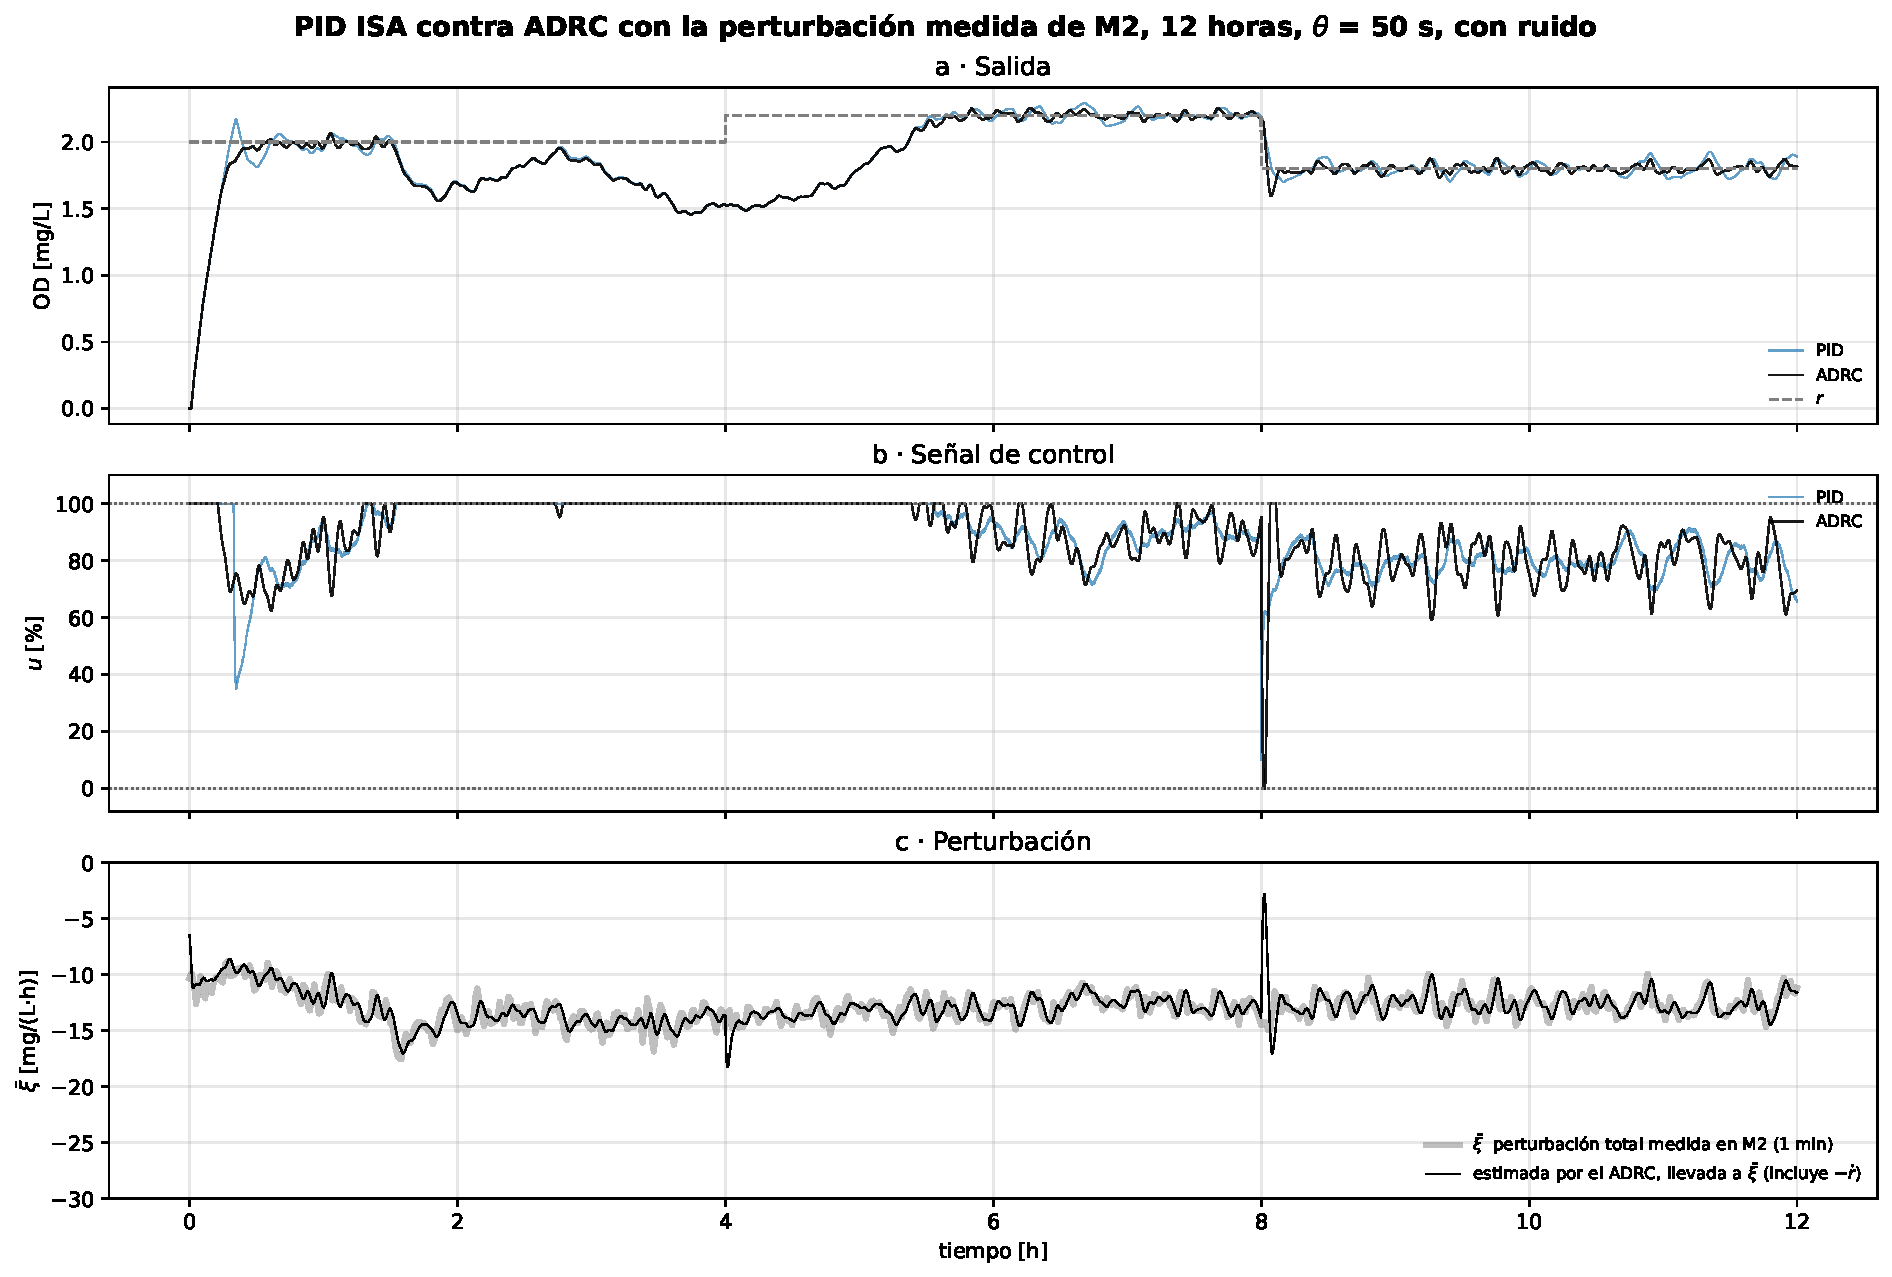
\includegraphics[width=\textwidth]{pid_adrc_perturbacion.pdf}
  \caption[PID ISA contra ADRC con la perturbación medida]{PID ISA contra
    ADRC con las 12~h de la perturbación medida en M2 de la Figura~\ref{fig:ident_perturbacion}, arranque desde
    $0$~mg/L y cambios de consigna a las 4 y a las 8~h, con $\theta = 50$~s y
    el soplador limitado entre $0$ y $100~\%$, con el ruido del sensor.
    (a) Salida. (b) Señal de control. (c) Perturbación total sobre la salida $\bar{\xi}$, medida y
    estimada por el observador del ADRC.}
  \label{fig:pid_adrc_perturbacion}
\end{figure}

\begin{table}[H]
\centering
\caption[Índices por cambio de consigna con la perturbación medida]{Índices
  de cada cambio de consigna con la perturbación medida, en una ventana de
  2~h desde el cambio. El IAE incluye el efecto de la perturbación en esa
  ventana.}
\label{tab:pid_cambios}
\renewcommand{\arraystretch}{1.3}
\resizebox{\textwidth}{!}{%
\begin{tabular}{lccccccc}
\toprule
 & & \multicolumn{2}{c}{\textbf{IAE sin ruido}} & \multicolumn{2}{c}{\textbf{IAE con ruido}} & \multicolumn{2}{c}{$\boldsymbol{M_p}$ \textbf{sin ruido}} \\
 & & \multicolumn{2}{c}{[mg$\cdot$s/L]} & \multicolumn{2}{c}{[mg$\cdot$s/L]} & \multicolumn{2}{c}{[\%]} \\
\cmidrule(lr){3-4} \cmidrule(lr){5-6} \cmidrule(lr){7-8}
\textbf{Cambio} [mg/L] & $\boldsymbol{t}$ [h] & \textbf{ADRC} & \textbf{PID} & \textbf{ADRC} & \textbf{PID} & \textbf{ADRC} & \textbf{PID} \\
\midrule
$0 \rightarrow 2{,}0$     & 0 & 1\,727 & 1\,793 & 1\,727 & 1\,793 & 3,2  & 8,6  \\
$2{,}0 \rightarrow 2{,}2$ & 4 & 2\,657 & 2\,631 & 2\,657 & 2\,631 & 24,9 & 24,6 \\
$2{,}2 \rightarrow 1{,}8$ & 8 & 247    & 303    & 247    & 303    & 51,8 & 25,1 \\
\bottomrule
\end{tabular}%
}
\end{table}


Con la perturbación medida se alcanza a ver un resultado parecido, aunque más ajustado. Con los
mismos valores de robustez ($M_s$), el IAE del PID en las 12~h es un poco mayor que el del ADRC,
$7\,333$ frente a $7\,043$~mg$\cdot$s/L; la mayor parte de ese error sale del tramo de la hora 1,5 a
la 5,5, donde el soplador se satura y ninguno de los dos puede sostener la consigna. Aun así, gracias
a sus esquemas de anti-\emph{windup}, los dos controladores aguantan ese tramo saturados y, cuando la
perturbación cede, el sistema vuelve a recuperar su comportamiento. En el arranque el PID se pasa más
(Tabla~\ref{tab:pid_cambios}); en la bajada a 1,8~mg/L de las 8~h, en cambio, es el ADRC el que más
se pasa, porque el cambio de consigna lleva su señal de control a 0~\% unos segundos y, con el retardo,
el OD baja de más. Con el ruido del sensor, el PID mueve mucho más el soplador, como ya se vio en el
escalón de consigna (Tabla~\ref{tab:pid_escalon}).

Por último, se probó el acondicionamiento de la referencia con el prefiltro y con la curva de Bézier,
usando la misma perturbación medida (Figura~\ref{fig:adrc_acond_perturbacion}). Con los dos, el
sistema llega más acondicionado a la referencia y aun así logra un buen rechazo de la perturbación,
porque el acondicionamiento queda por fuera del lazo; en la bajada de las 8~h el sobrepico baja a la
tercera parte y queda por debajo del del PID. Con el prefiltro, el sistema se comporta más
parecido a uno de primer orden, debido a la cancelación del cero; con el Bézier la respuesta es más
suave, a cambio de un tiempo final de $2\,\tau$, que se puede acortar si se quiere una respuesta más
rápida.


\begin{figure}[H]
  \centering
  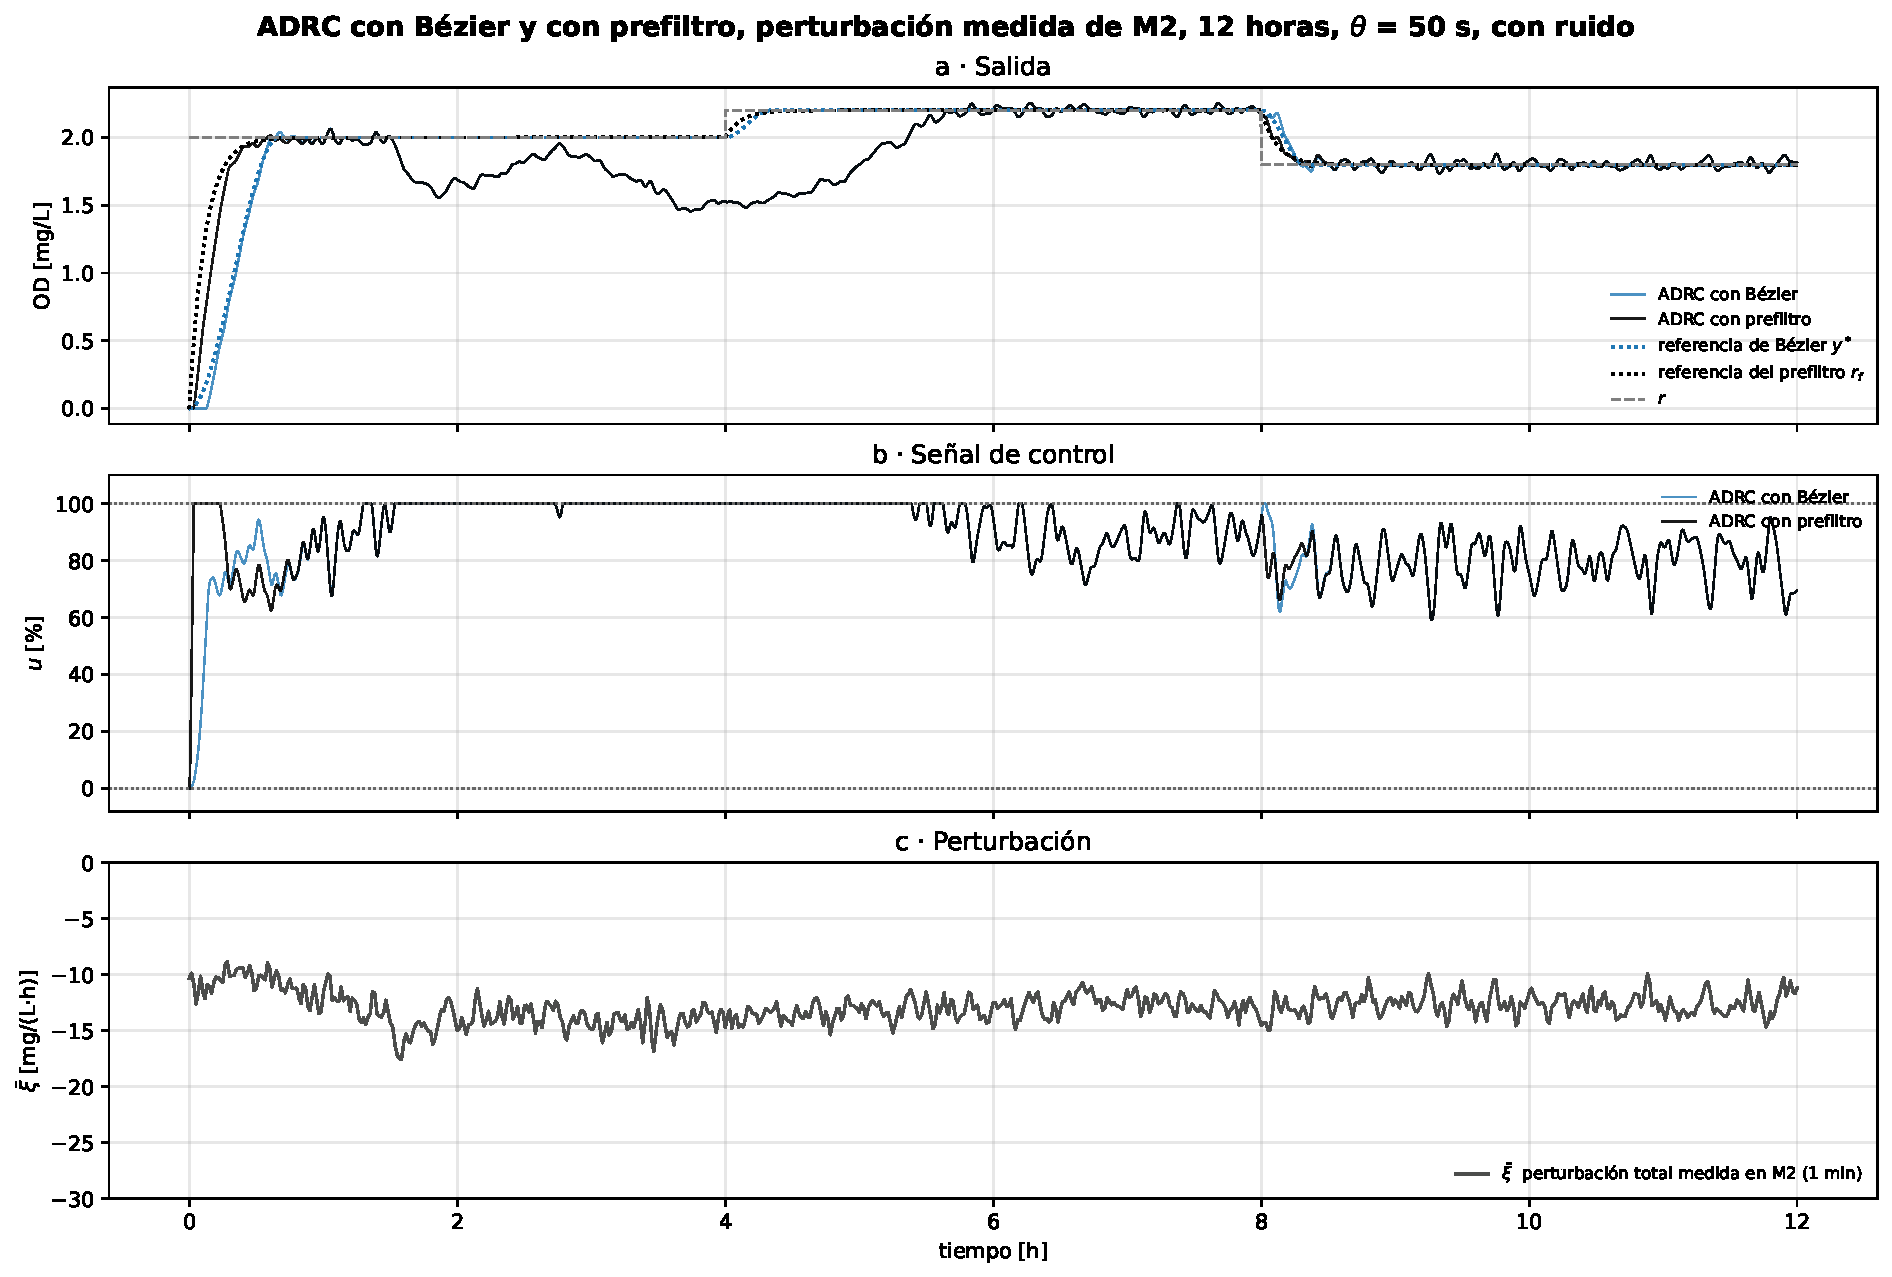
\includegraphics[width=\textwidth]{adrc_acond_perturbacion.pdf}
  \caption[ADRC con Bézier y con prefiltro, con la perturbación medida]{ADRC con la referencia
    acondicionada por la curva de Bézier y por el prefiltro, con la misma perturbación medida,
    consignas, retardo y ruido de la Figura~\ref{fig:pid_adrc_perturbacion}. (a) Salida, con la referencia
    de Bézier y la del prefiltro en punteado. (b) Señal de
    control. (c) Perturbación total sobre la salida $\bar{\xi}$, medida.}
  \label{fig:adrc_acond_perturbacion}
\end{figure}

%--------------------------------------------------------------------
\section{Comparación de desempeños}
\label{sec:pid_mejores}

Con el mismo procedimiento de sintonía se puede obtener un controlador con mejor desempeño que el
ADRC, sin que la señal de control llegue al $100~\%$ (Figura~\ref{fig:pid_mejores},
Tabla~\ref{tab:pid_mejores}): un PI ($T_d = 0$), sintonizado de forma muy similar al PID. Primero se
ajusta $K_p$ para que el salto inicial no supere el $40~\%$; como el PI no tiene derivada, todo el salto
es proporcional y queda $K_p = 200~\%/(\mathrm{mg/L})$. Luego se ajusta $T_i$ para que tenga la misma
robustez que el ADRC, en este caso el mismo margen de fase sin retardo, $65{,}8^{\circ}$, porque con la
misma $M_s$ queda casi inestable con retardo. Resulta
$T_i = 188$~s. Con más o menos la misma robustez, este PI sigue la consigna casi igual que el ADRC y
rechaza mejor la perturbación; ahora bien, sin retardo sigue teniendo un mayor sobrepico. Aun así, para
este tipo de plantas de primer orden, un PI solo puede ser incluso mejor que un PID. En la
Figura~\ref{fig:pid_mejores_sensibilidad} se ve por qué: el PI atenúa más las perturbaciones de baja
frecuencia y, con retardo, su pico de sensibilidad es menor que el del ADRC, a cambio de dejar pasar más
ruido.

\begin{figure}[H]
  \centering
  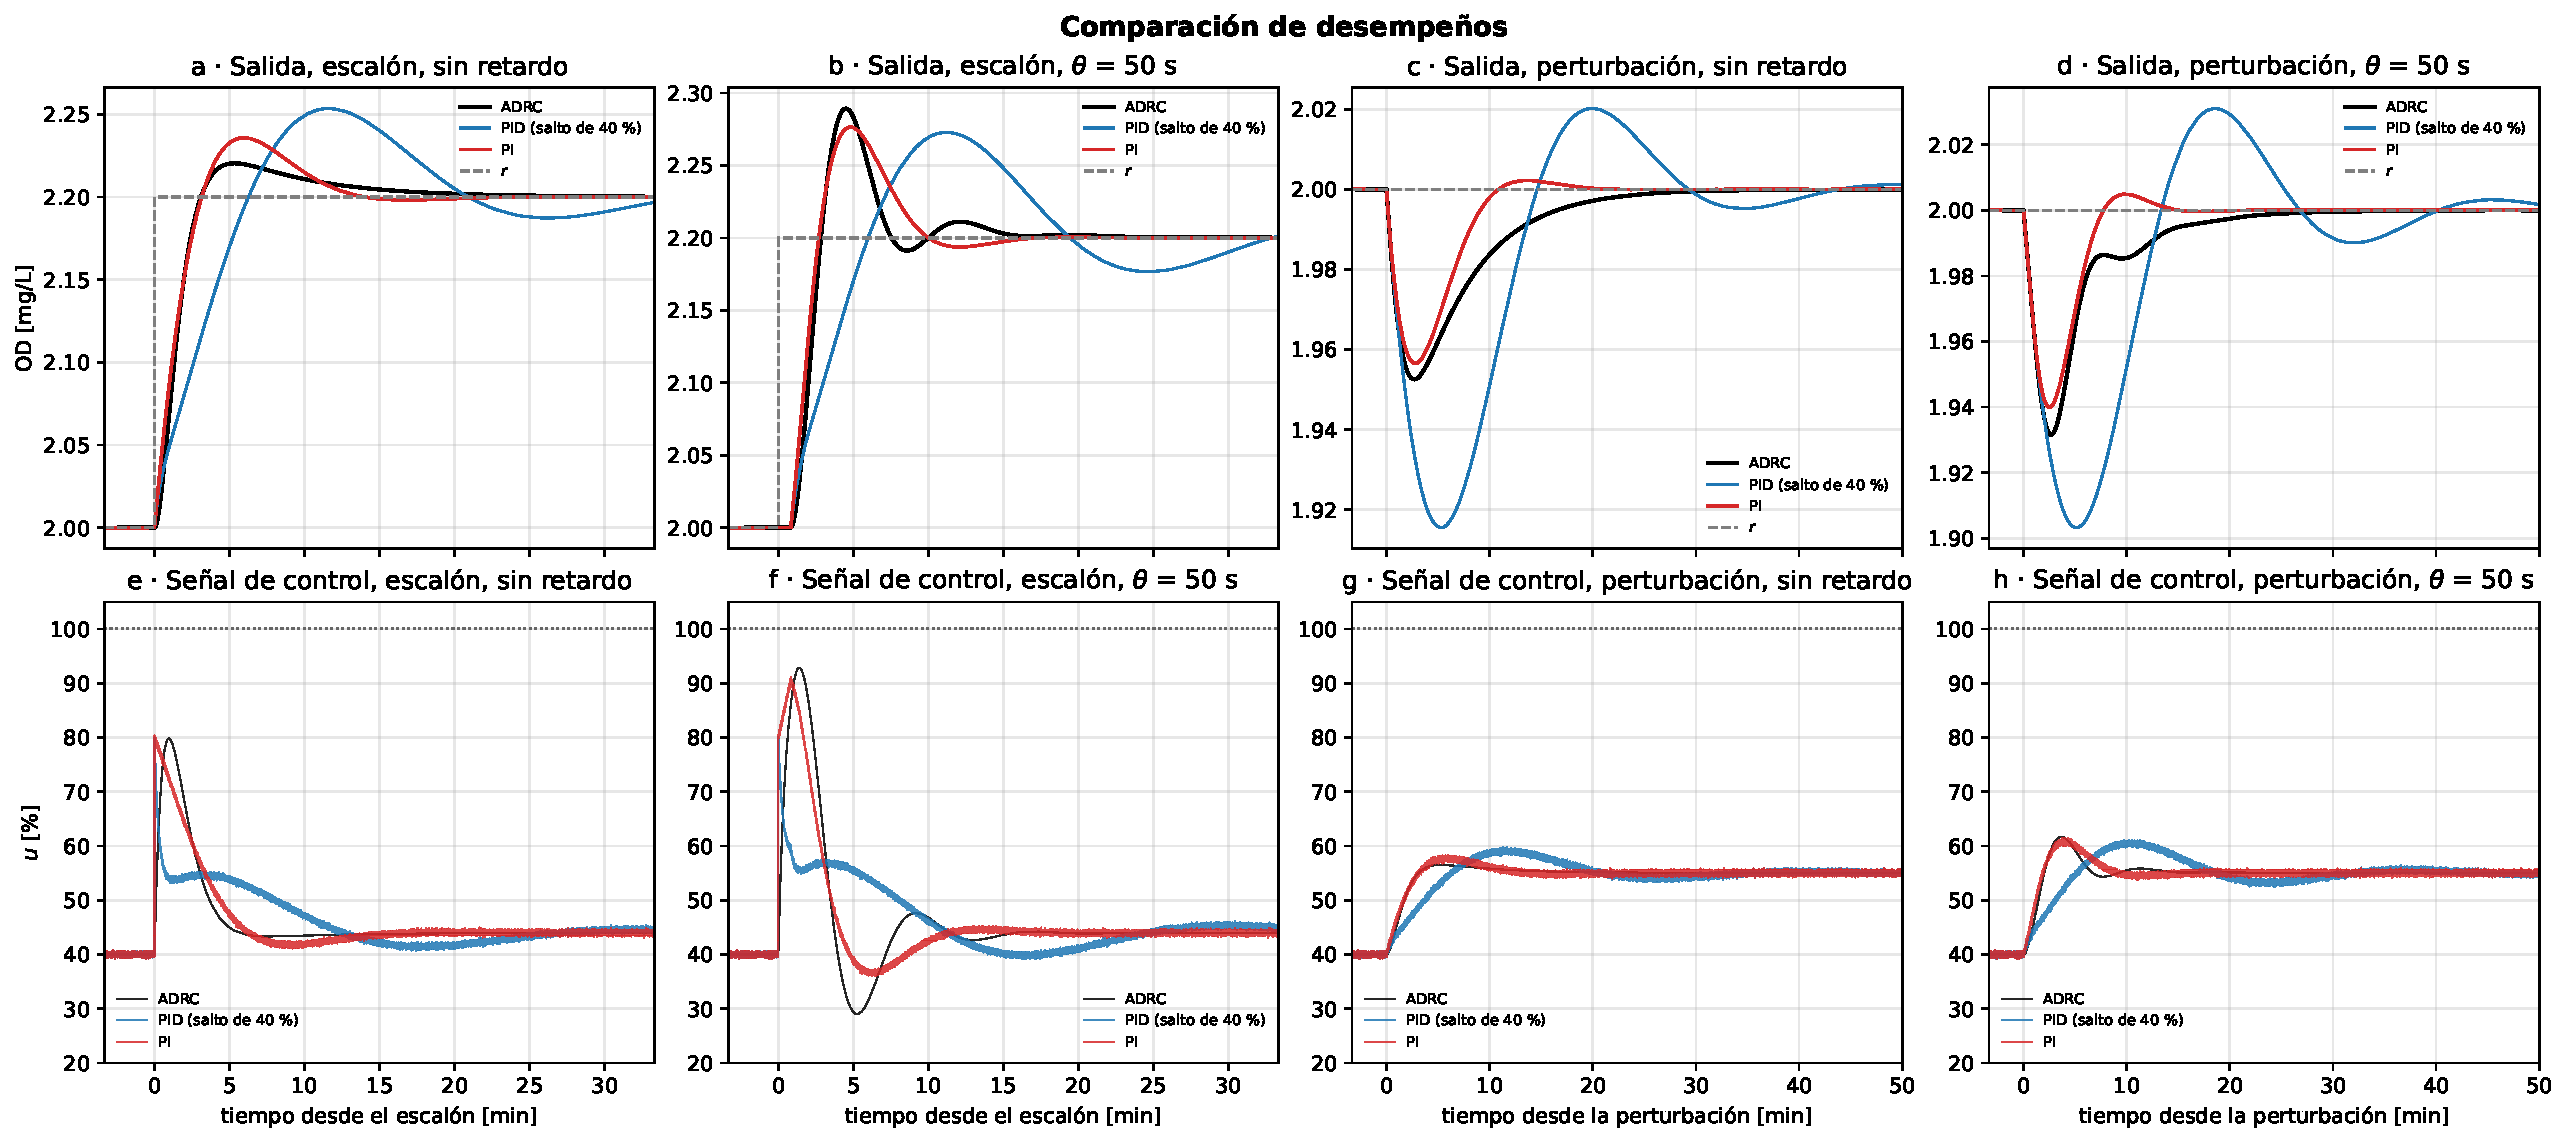
\includegraphics[width=\textwidth]{pid_mejores.pdf}
  \caption[Comparación de desempeños]{ADRC, PID \eqref{eq:pid_ganancias} y PI
    ($K_p = 200~\%/(\mathrm{mg/L})$, $T_i = 188$~s), con el ruido del sensor y
    el soplador limitado entre $0$ y $100~\%$. (a), (b), (e) y (f) Escalón de consigna de $2{,}0$ a
    $2{,}2$~mg/L; (c), (d), (g) y (h) perturbación de entrada $\varepsilon = -15~\%$. En cada par, sin retardo
    y con $\theta = 50$~s; arriba, la salida, y abajo, la señal de control.}
  \label{fig:pid_mejores}
\end{figure}

\begin{table}[H]
\centering
\caption[Robustez y desempeño en la comparación de desempeños]{Robustez y desempeño del ADRC, el PID y el
  PI, sin retardo y con $\theta = 50$~s (Tabla~\ref{tab:metricas}). Los
  índices se miden sin ruido, salvo $\sigma_u$.}
\label{tab:pid_mejores}
\renewcommand{\arraystretch}{1.3}
\resizebox{\textwidth}{!}{%
\begin{tabular}{lcccccccc}
\toprule
 & $\boldsymbol{M_s}$ & \textbf{MF} & \textbf{IAE consigna} & \textbf{ITAE consigna} & $\boldsymbol{M_p}$ & \textbf{IAE rechazo} & $\boldsymbol{u_{\max}}$ & $\boldsymbol{\sigma_u}$ \\
 & $\theta = 0$ / $50$~s & $\theta = 0$ / $50$~s & [mg$\cdot$s/L] & [mg$\cdot$s$^2$/L] & [\%] & [mg$\cdot$s/L] & [\%] & [\%] \\
\midrule
ADRC            & 1,20 / 2,32 & $65{,}8^{\circ}$ / $36{,}0^{\circ}$ & 26,9 / 42,7 & 6\,909 / 9\,308   & 10,2 / 44,6 & 24,8 / 24,8 & 80 / 93  & 0,009 \\
PID             & 1,20 / 1,59 & $50{,}0^{\circ}$ / $37{,}5^{\circ}$ & 69,2 / 88,4 & 40\,127 / 56\,567 & 26,7 / 36,4 & 58,8 / 70,2 & 80 / 80  & 0,220 \\
PI              & 1,00 / 1,73 & $65{,}8^{\circ}$ / $38{,}6^{\circ}$ & 28,3 / 41,0 & 6\,802 / 8\,665   & 17,9 / 38,2 & 15,6 / 16,5 & 80 / 91  & 0,220 \\
\bottomrule
\end{tabular}%
}
\end{table}

\begin{figure}[H]
  \centering
  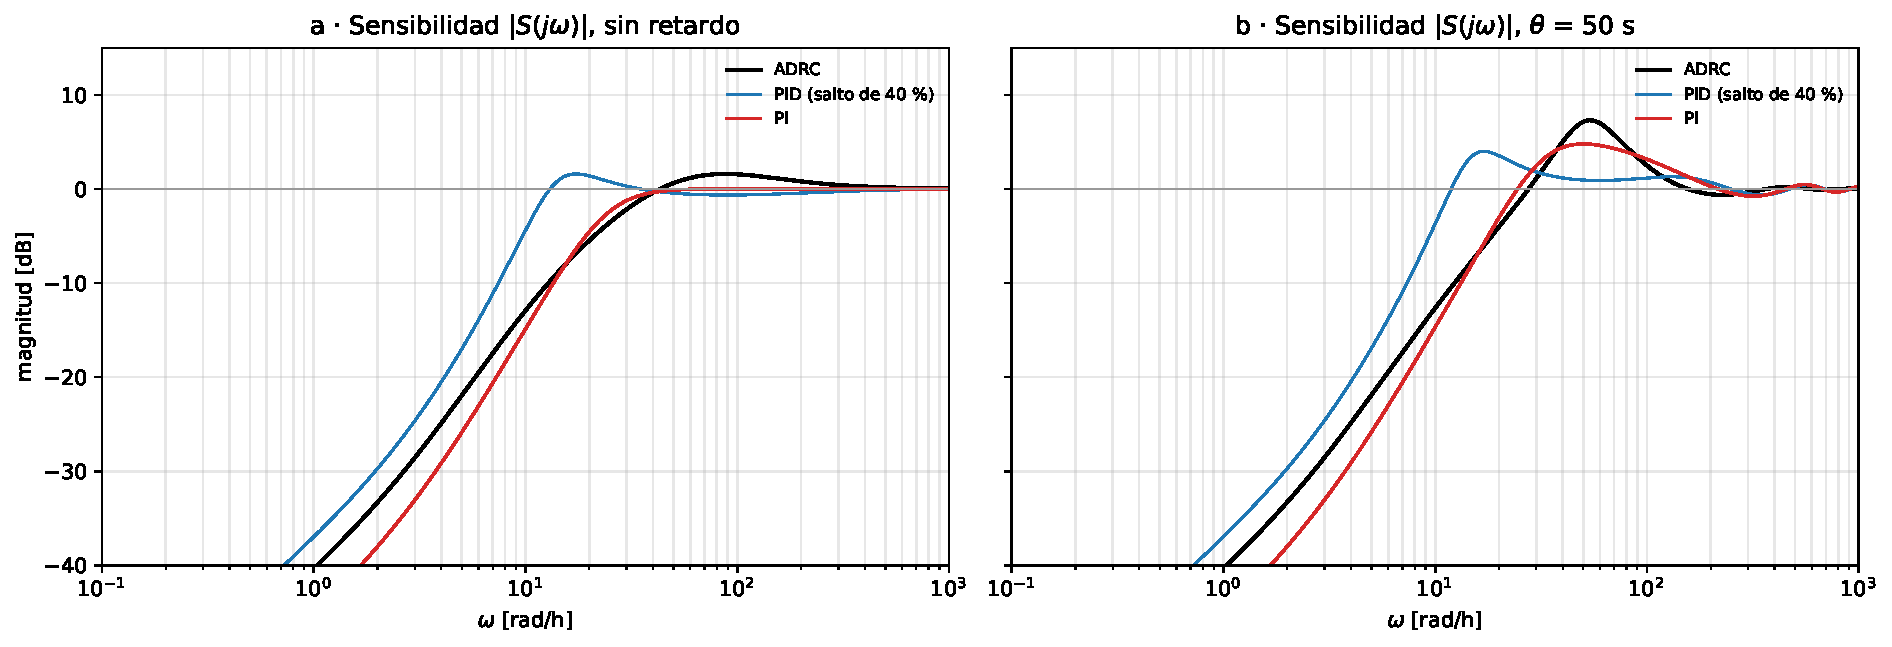
\includegraphics[width=\textwidth]{pid_mejores_sensibilidad.pdf}
  \caption[Sensibilidad en la comparación de desempeños]{Sensibilidad $|S(j\omega)|$ del ADRC, el PID y el
    PI: (a) sin retardo y (b) con $\theta = 50$~s.}
  \label{fig:pid_mejores_sensibilidad}
\end{figure}

Ahora bien, al introducir el retardo se ve que todos tienen más o menos el mismo margen de fase, y el
del ADRC es el más bajo, con $36{,}0^{\circ}$ (Tabla~\ref{tab:pid_mejores}). Pero el ADRC tiene un mejor
comportamiento al arrancar la señal de control, porque la sube de forma
suave, sin el salto del PI ni del PID en el cambio de consigna (Figura~\ref{fig:pid_mejores}(e) y (f)).
Y en el ruido, el ADRC casi no lo deja pasar, mientras que el PI y el PID sí
(Figura~\ref{fig:pid_mejores}(e) a (h)). La diferencia entre este ADRC y el PI está en su filtro en
cascada: el ADRC se puede escribir como un PI con un filtro del error \eqref{eq:gpi_pi_filtro}, y es ese
filtro el que no deja pasar el ruido. Además, el ADRC puede llegar a superarlo en seguimiento cuando la referencia es de mayor orden:
con solo subir el grado del modelo de la perturbación se sigue mejor, tanto con el ESO como con el GPI
(Tabla~\ref{tab:gpi_conteo}), y conceptualmente es más simple. 